\begin{frame}
\frametitle{Electronic Flight Bags}
\begin{center}
Aeronautical Data and Information
\end{center}
\end{frame}

\begin{frame}
\frametitle{Aeronautical Data and Information}
\begin{block}{Aviation, Navigation and Geodesy}
\begin{itemize}
\item<1-> I have not taken any serious programming steps toward solving this problem.
\item<2-> This stuff gets me a bit ranty.
\item<3-> Here is the problem.
\end{itemize}
\end{block}
\end{frame}

\begin{frame}
\frametitle{CASR 175}
\begin{block}{What is CASR 175 about?}
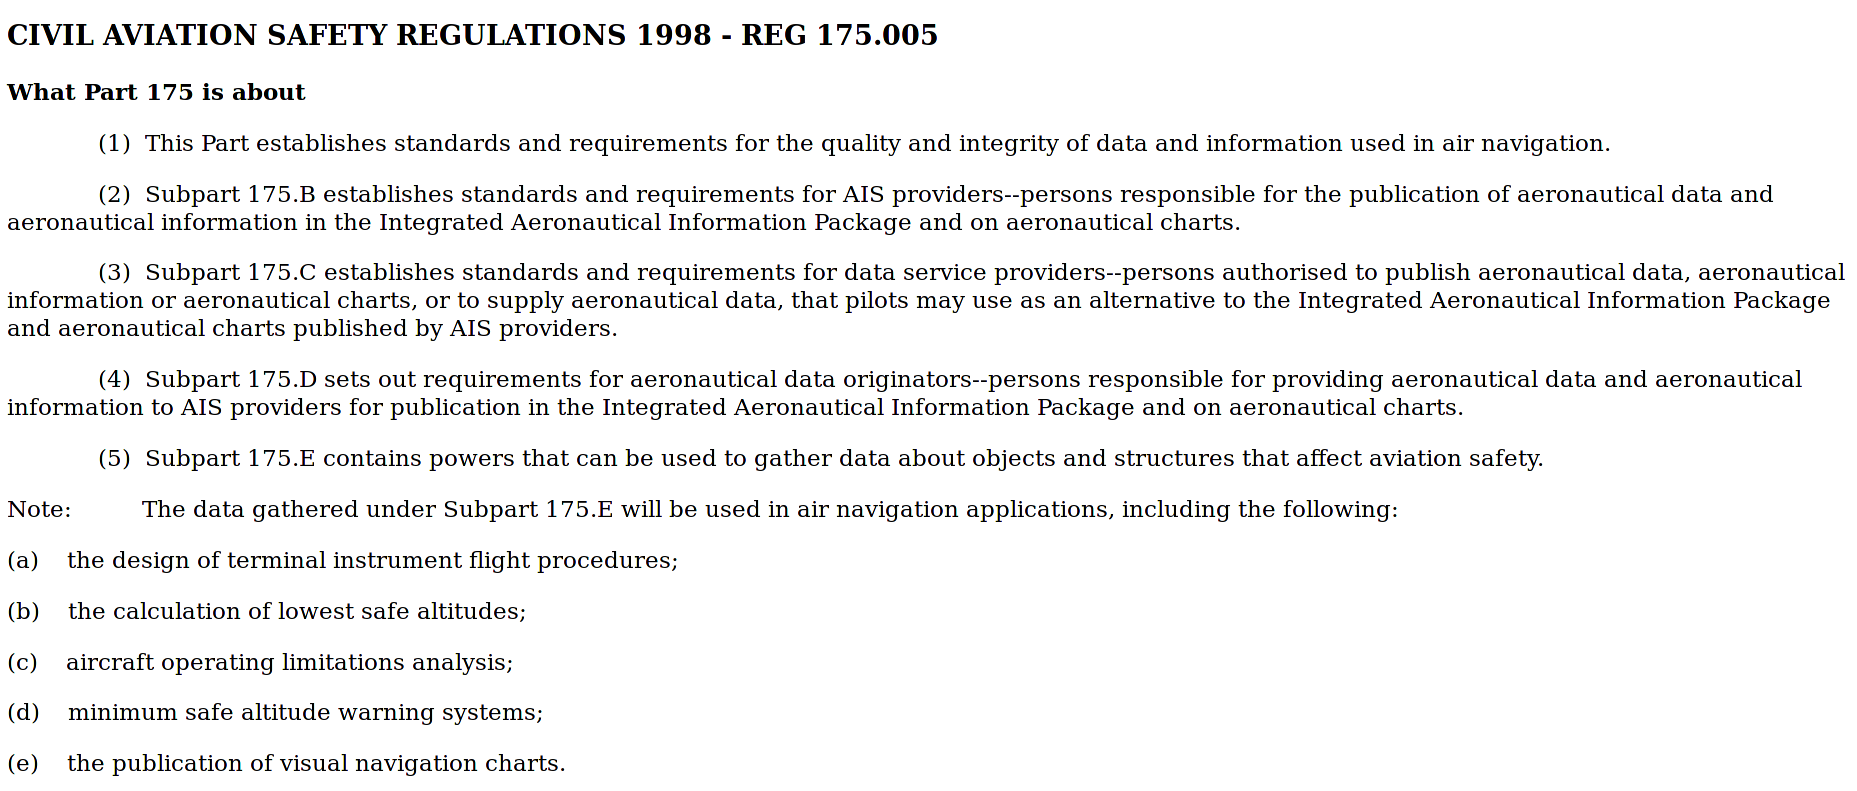
\includegraphics[height=0.5\textheight]{image/casr175_005.png}
\end{block}
\par
``(e) the publication of visual navigation charts.''
\end{frame}

\begin{frame}
\frametitle{CAR1988 REG 133(1)(h) \emph{moved to CASR1998 REG 175}}
\scriptsize
\begin{block}{CAR1988 REG 133(1)(h)}
The pilot in command of an aircraft must not commence a flight if he or she has not received evidence, and taken such action as is necessary to ensure, that:
\par
\ldots
\par
(h)  the aeronautical data and aeronautical information mentioned in subregulation (1A) is carried in the aircraft and is readily accessible to the flight crew.
\end{block}
\par
\end{frame}

\begin{frame}
\frametitle{VTC/VNC}
\begin{block}{This is a Brisbane Visual Terminal Chart (VTC)}
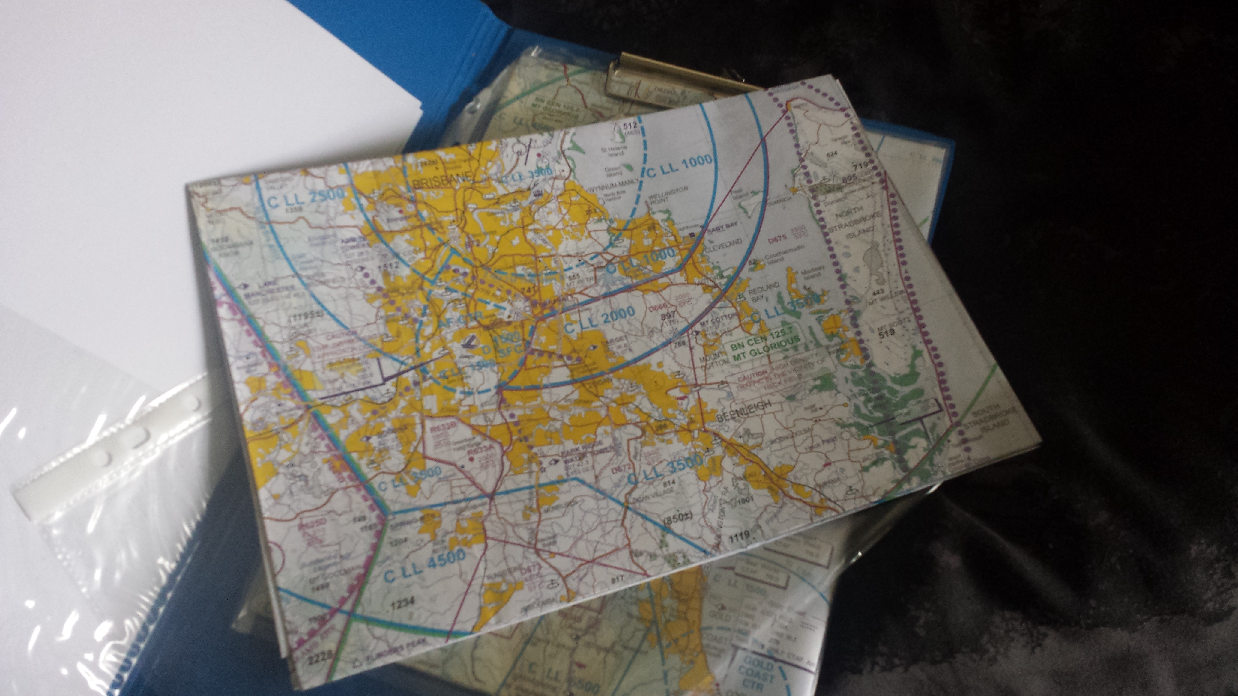
\includegraphics[height=0.3\textheight]{image/vtc.png}
\begin{itemize}
\item<1-> It unfolds out to 500mm x 1000mm.
\item<2-> Updated every 3 months (approx).
\item<3-> Similar to another chart; VNC.
\item<4-> It is physically impossible for these documents to be ready accessible. \tiny{Let's pretend.}
\end{itemize}
\end{block}
\end{frame}

\begin{frame}
\frametitle{VTC/VNC}
\begin{block}{Under CAR1988 REG 133(1)(h)}
\begin{itemize}
\item<1-> I am required to carry these charts on \emph{every flight}.
\item<2-> I don't \emph{actually} read them, because it is physically impossible in-flight.
\item<3-> I do, however, memorise the important parts.
\end{itemize}
\end{block}
\end{frame}

\begin{frame}
\frametitle{VTC/VNC}
\begin{block}{Surely these exist in electronic format?}
Why yes, they do.
\end{block}
\end{frame}

\begin{frame}
\frametitle{VTC/VNC}
\large
\begin{center}
but
\end{center}
\end{frame}

\begin{frame}
\frametitle{CASR1998 REG 175.145(1)}
\begin{block}{AIS providers--publication of aeronautical charts relating to areas etc. outside authority}
(1) This regulation applies if an AIS provider publishes an aeronautical chart that includes aeronautical data or aeronautical information that relates to an area, aerodrome, airspace or ATS route not covered by the provider's certificate.
\end{block}
\end{frame}

\begin{frame}
\frametitle{CASR1998 REG 175.145(1)}
\large
\begin{center}
No problem.
\par
I will use approved electronic AIS aeronautical charts.
\end{center}
\end{frame}

\begin{frame}
\frametitle{CASR1998 REG 175.145(1)}
\begin{center}
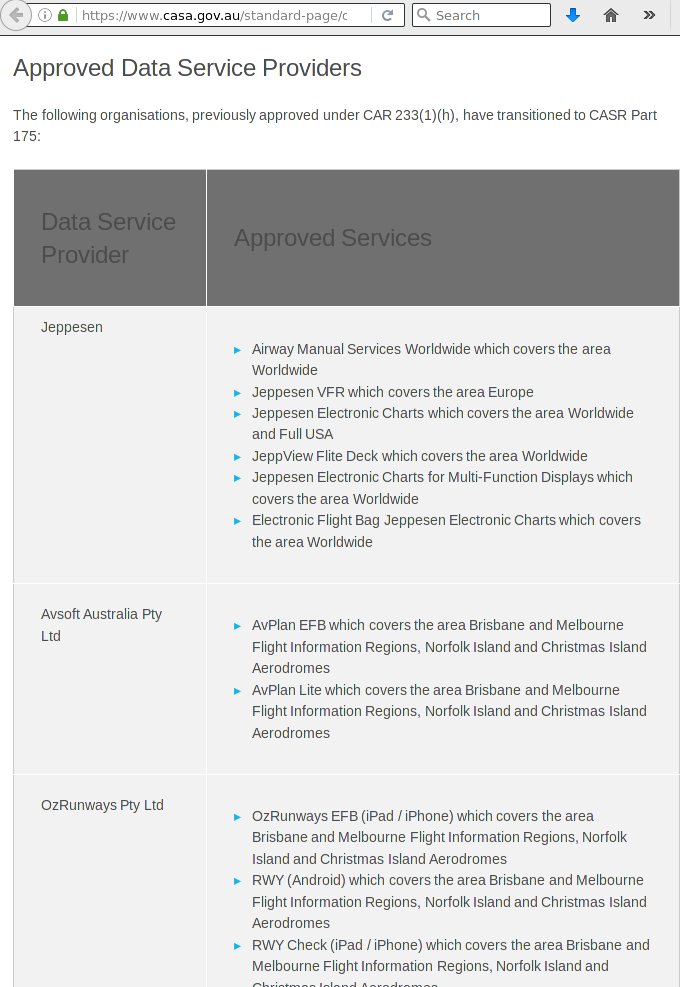
\includegraphics[height=0.8\textheight]{image/casa-approved-data-service-providers.png}
\end{center}
\end{frame}

\begin{frame}
\frametitle{CASR1998 REG 175.145(1)}
\large
\begin{center}
but
\end{center}
\end{frame}

\begin{frame}
\frametitle{CASR1998 REG 175.145(1)}
\large
\begin{center}
the paper charts are the authoritative data source.
\end{center}
\end{frame}

\begin{frame}
\frametitle{CASR1998 REG 175.145(1)}
\begin{block}{let's fly across .png files}
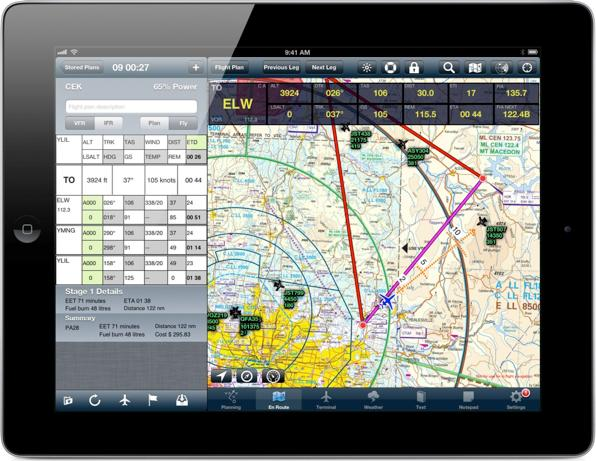
\includegraphics[height=0.5\textheight]{image/avplan-screenshot.jpg}
\end{block}
\end{frame}

\begin{frame}
\frametitle{CASR1998 REG 175.145(1)}
\begin{block}{that do not georectify}
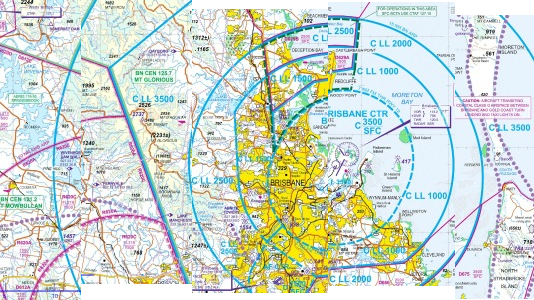
\includegraphics[height=0.5\textheight]{image/vtc-georectification.png}
\end{block}
\end{frame}

\begin{frame}
\frametitle{CASR1998 REG 175}
\begin{block}{is accuracy important?}
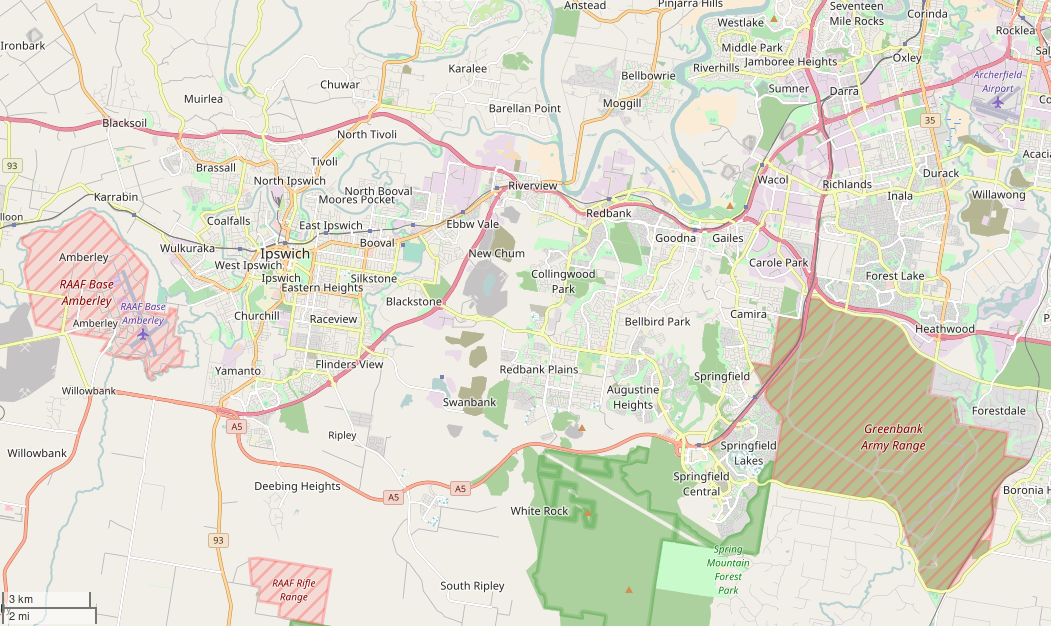
\includegraphics[height=0.5\textheight]{image/map-amberley-greenbank.png}
\end{block}
\end{frame}

\begin{frame}
\frametitle{CASR1998 REG 175}
\begin{block}{Yes}
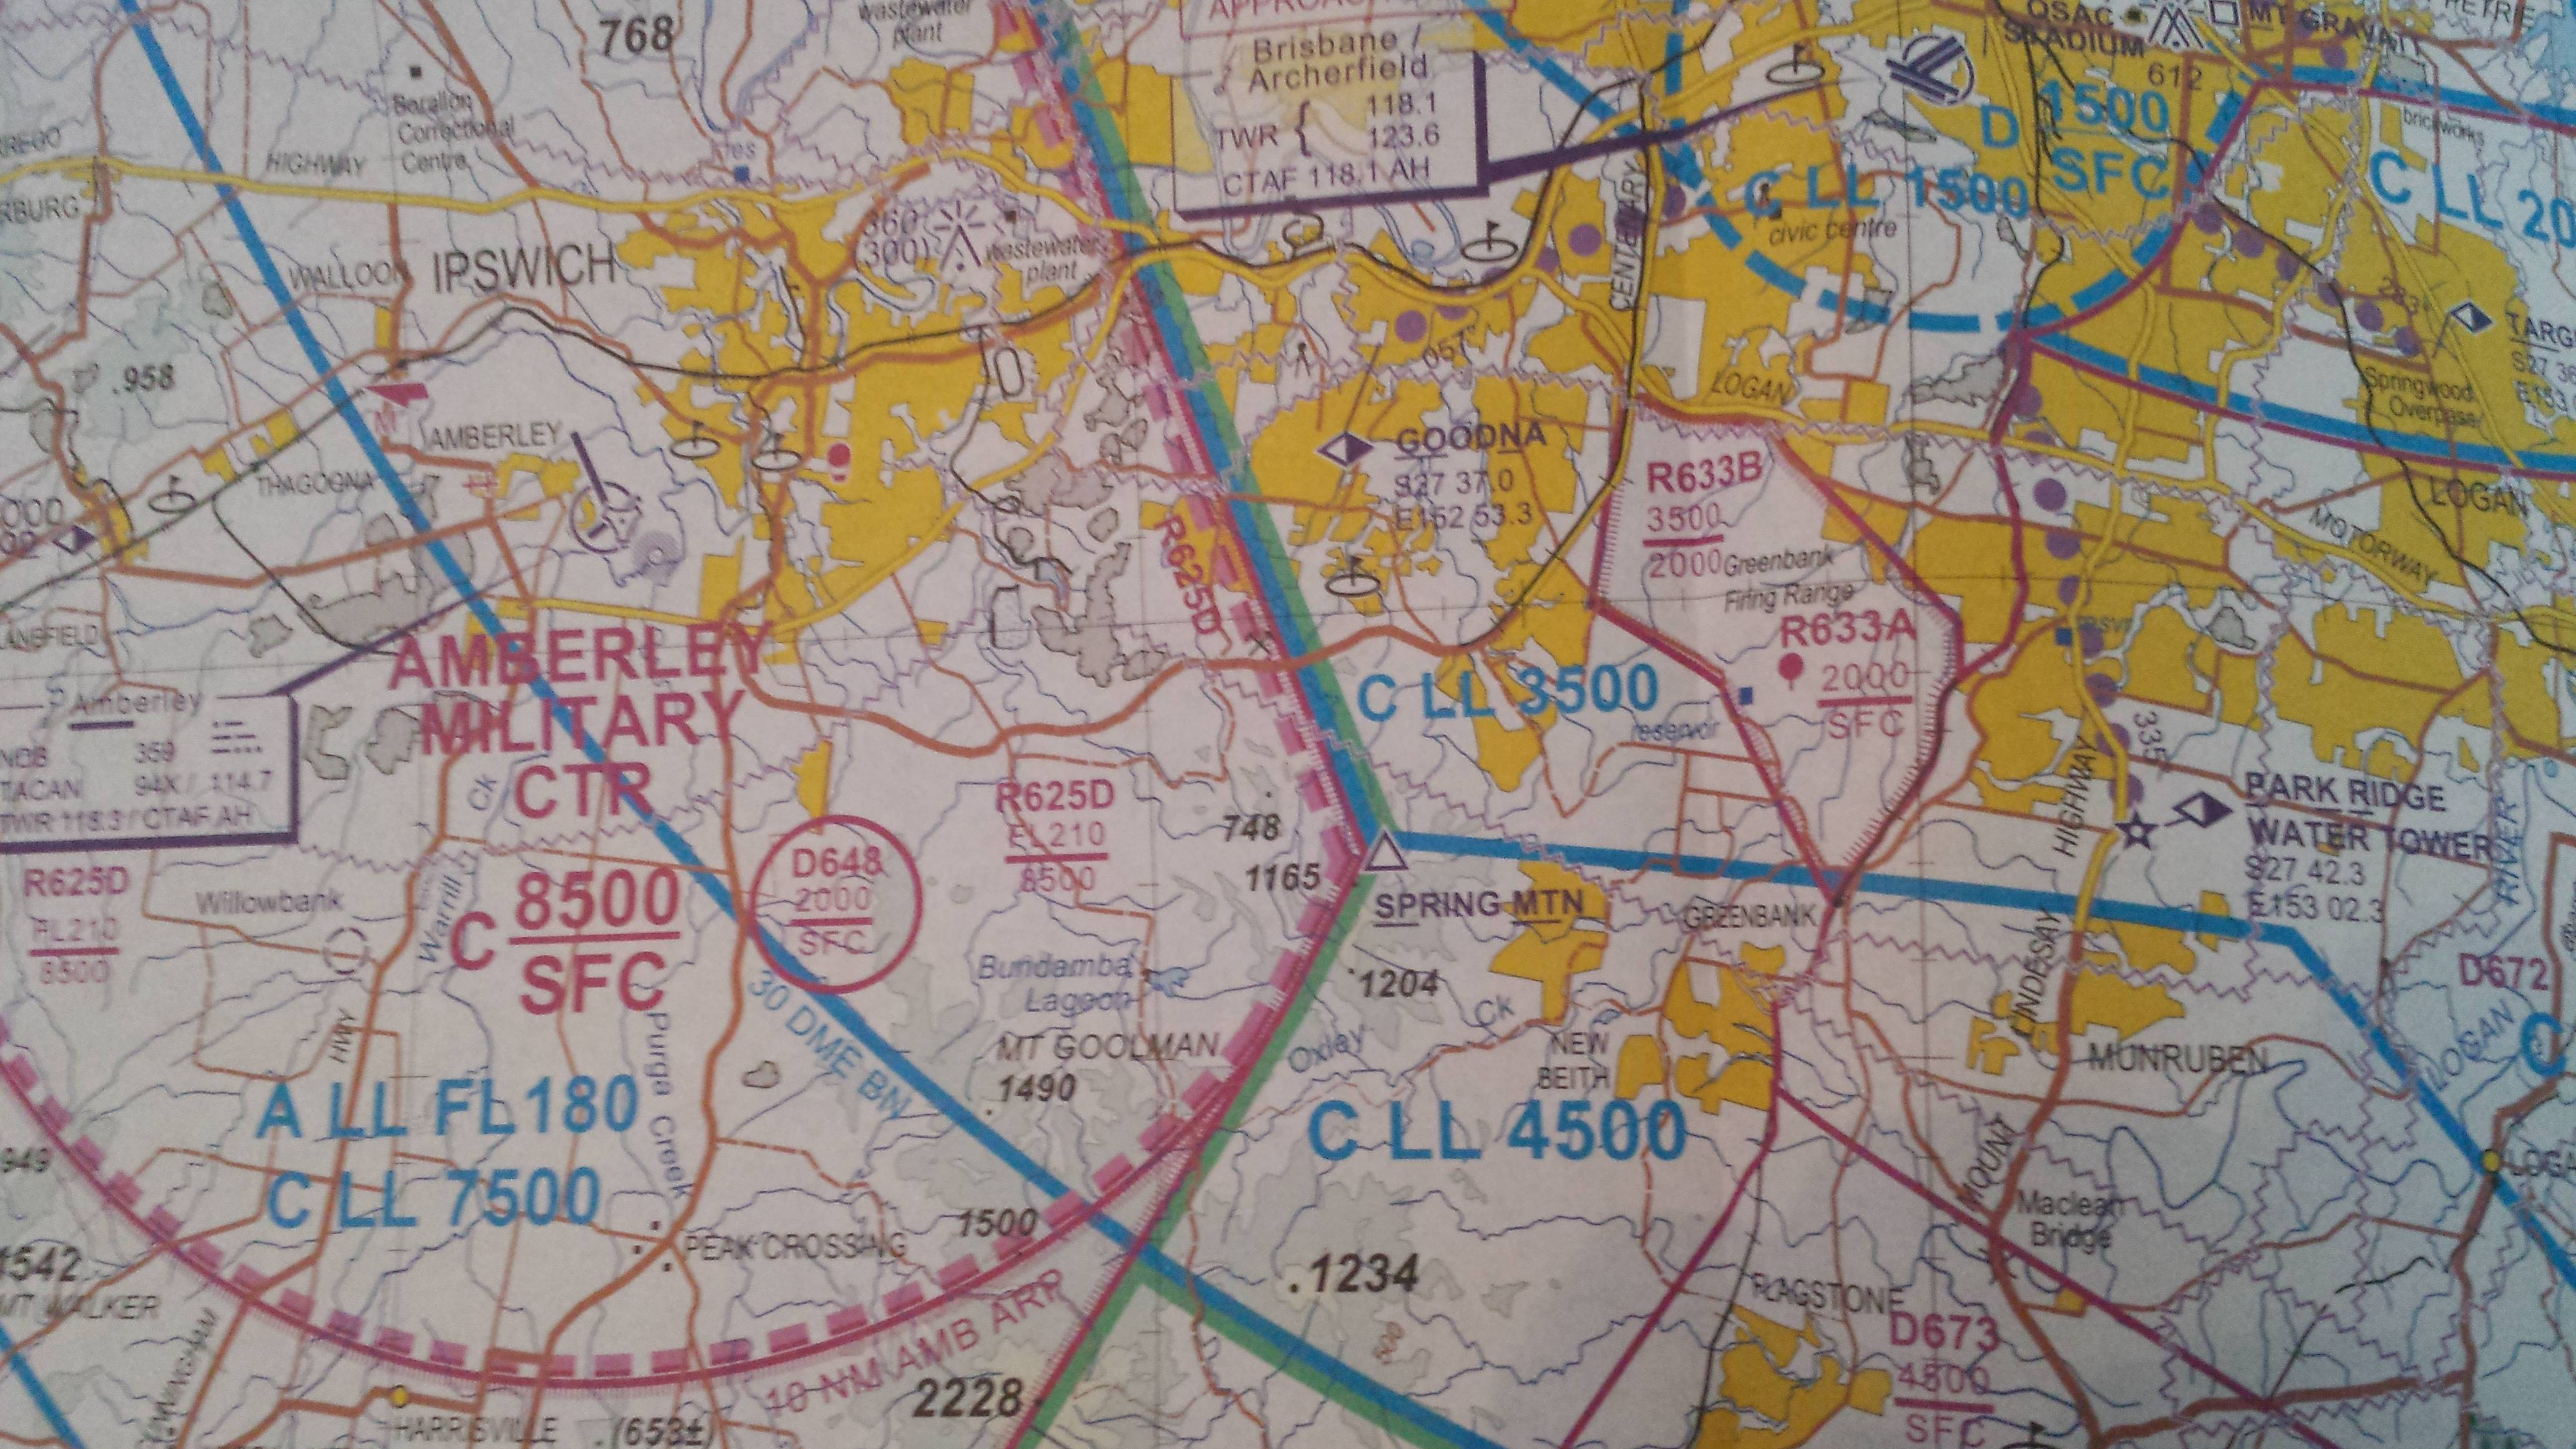
\includegraphics[height=0.5\textheight]{image/vtc-amberley-greenbank.jpg}
\begin{itemize}
\item \tiny{Amberley RAAF is conditionally \textbf{RA2}}
\item \tiny{Greenbank Army is \textbf{RA3} SFC to 2000}
\end{itemize}
\end{block}
\end{frame}

\begin{frame}
\frametitle{CASR1998 REG 175}
\begin{block}{My nightmares are made of this stuff}
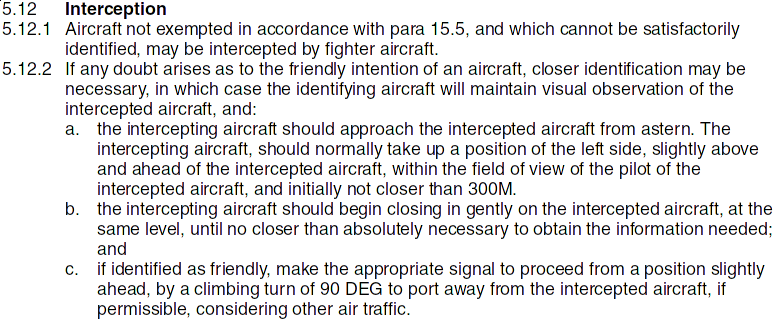
\includegraphics[height=0.5\textheight]{image/ersa-interception.png}
\end{block}
\end{frame}

\begin{frame}
\frametitle{CASR1998 REG 175}
\begin{block}{Alternatively}
\begin{center}
Use uncertificated aeronautical data with restrictions on operations.
\end{center}
\end{block}
\end{frame}

\begin{frame}
\frametitle{uncertificated aeronautical data}
\large
\begin{center}
but
\end{center}
\end{frame}

\begin{frame}
\frametitle{New Zealand CAA}
\begin{block}{Fatal Accident Report ZK-SML, Mount Duppa, 09 April 2011. \textbf{CFIT}}
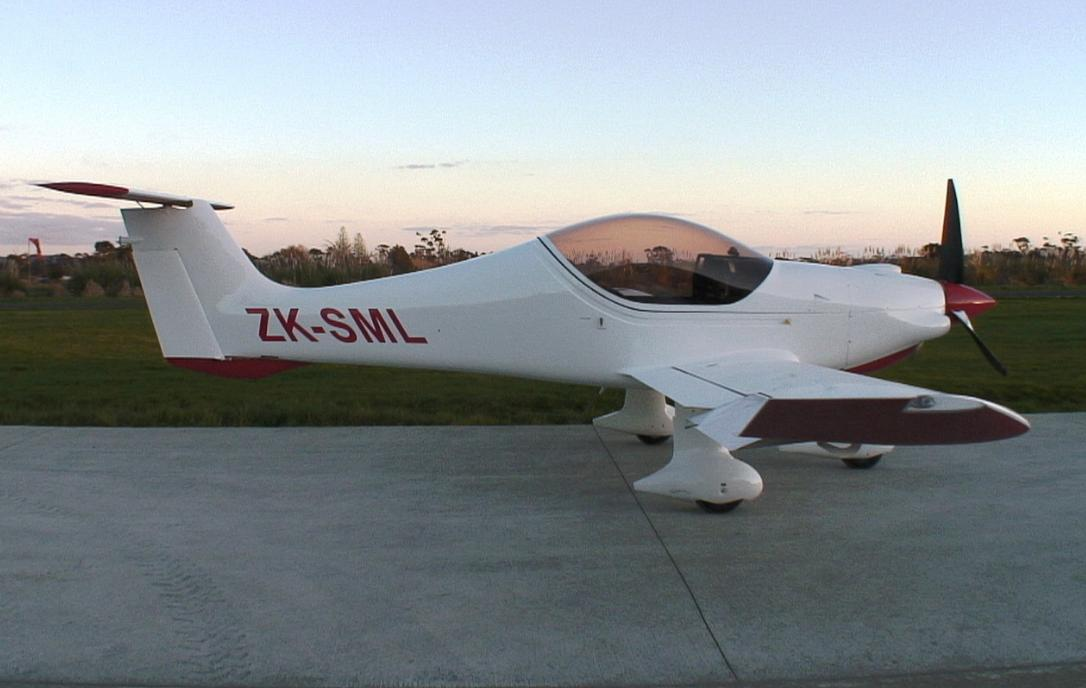
\includegraphics[height=0.5\textheight]{image/zk-sml.jpg}
\end{block}
\end{frame}

\begin{frame}
\frametitle{ZK-SML}
\begin{block}{VFR into IMC \emph{likely}}
\begin{itemize}
\item<1-> VFR into IMC is a dangerous flight condition where the pilot has lost outside visual reference e.g. due to weather
\item<2-> It is particularly dangerous if the pilot is untrained and/or the aircraft is ill-equipped to handle instrument conditions
\item<3-> ZK-SML is a light, VFR only, experimental aircraft with \textbf{lots} of modern technology onboard
\item<4-> \tiny{please excuse me if I begin appearing a little angry}
\end{itemize}
\end{block}
\end{frame}

\begin{frame}
\frametitle{ZK-SML}
\begin{block}{Accident Report excerpt \emph{1.16.1}}
\begin{quote}
Assistance was sought from the New Zealand agent for the MGL Avionics EFIS system installed in the aircraft.  While reviewing the aircraft's flight path based on the SSR data on a computer based simulator, two major errors in the EFIS navigation software were discovered. 
\end{quote}
\end{block}
\end{frame}

\begin{frame}
\frametitle{ZK-SML}
\begin{block}{Accident Report excerpt \emph{1.16.2}}
\begin{quote}
It was found that the moving map display did not accurately display the 3717 feet spot height for Mount Duppa.  Due to the positioning of a map join which passes through the `3', the spot height for Mount Duppa was corrupted and was displayed as 1717 feet.  Refer to the spot height next to the aircraft symbol on the map display in figure 2. 
\end{quote}
\end{block}
\end{frame}

\begin{frame}
\frametitle{ZK-SML}
\begin{block}{Accident Report excerpt \emph{Figure 2}}
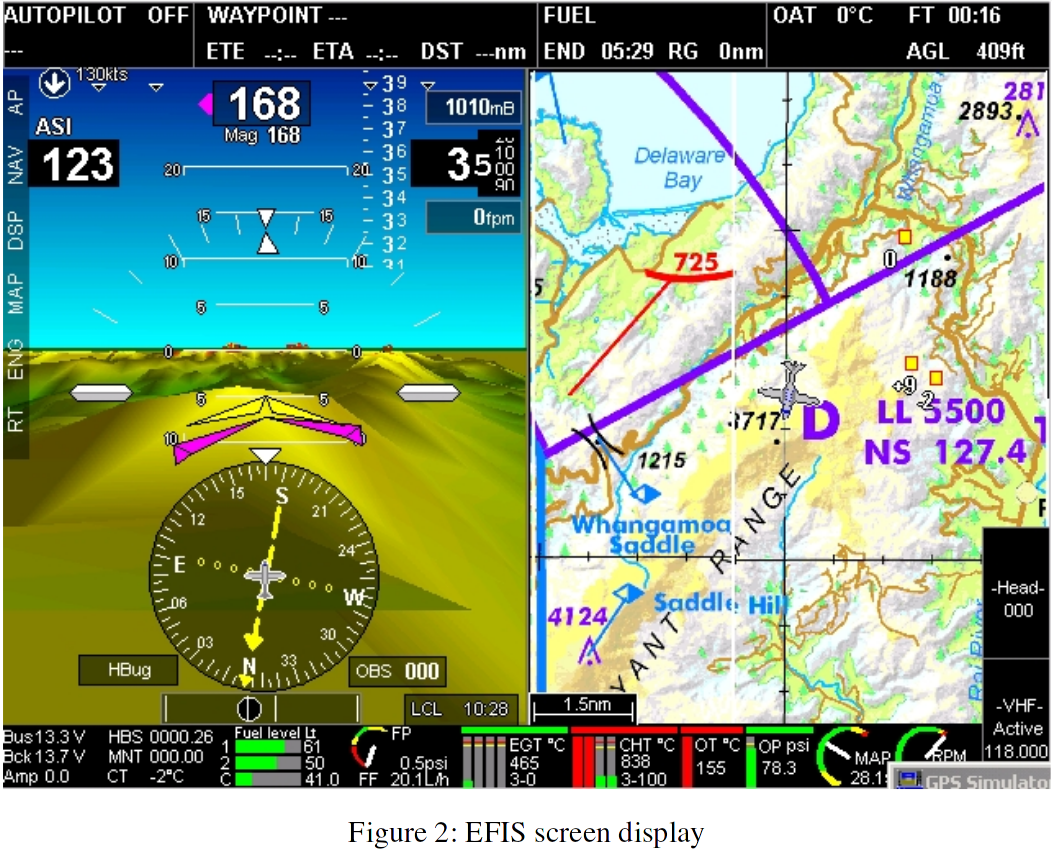
\includegraphics[height=0.7\textheight]{image/zk-sml-map.png}
\end{block}
\end{frame}

\begin{frame}
\frametitle{ZK-SML}
\begin{block}{Accident Report excerpt \emph{1.16.3}}
\begin{quote}
A further error affected the synthetic terrain display and warnings.  An error of approximately 600 feet existed between the actual terrain height and the modelled terrain height in the EFIS terrain data base for the accident flight.  This error led to the synthetic terrain displaying terrain indications associated with the modelled terrain of approximately 600 feet lower than the actual terrain. 
\end{quote}
\end{block}
\end{frame}

\begin{frame}
\frametitle{ZK-SML}
\begin{block}{Accident Report excerpt \emph{1.16.4}}
\begin{quote}
The New Zealand agent for MGL Avionics Ltd immediately contacted the manufacturer and reported these errors.  It transpired that the New Zealand terrain data used by MGL Avionics Ltd was based on publically available terrain data available from NASA.  The NASA terrain data used averages of the surrounding spot heights which had induced errors leading to the under reading of the actual terrain heights displayed on the EFIS. 
\end{quote}
\end{block}
\end{frame}

\begin{frame}
\frametitle{ZK-SML}
\begin{block}{Accident Report}
If you wish to share my frustration, the full report will blow your mind.
\end{block}
``Fatal Accident Report CAA Occ no: 11/1504''
\end{frame}

\begin{frame}
\frametitle{Programming}
\begin{block}{What programming tools can help here?}
\begin{itemize}
\item<1-> revision control with contributions from \emph{arbitrary sources}
\item<2-> digital signature on authoritative aeronautical data
\item<3-> queryable data structures for implementing automated systems
\item<4-> ``tell the pilot everything they need to know \textbf{and nothing more}''
\end{itemize}
\end{block}
\end{frame}

\begin{frame}
\frametitle{Programming}
\begin{block}{Because it's not like airservices gets it right}
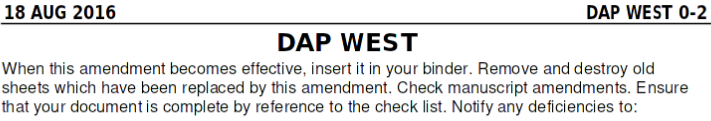
\includegraphics[height=0.18\textheight]{image/dap-amendment.png}
\end{block}
\end{frame}

\begin{frame}
\frametitle{Programming}
\begin{block}{This is how airservices does patches and pull requests}
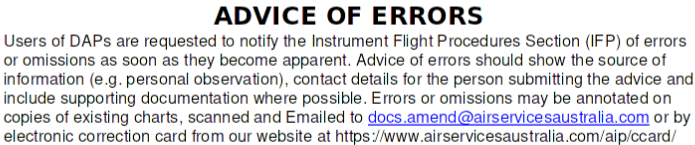
\includegraphics[height=0.2\textheight]{image/dap-errors.png}
\end{block}
\end{frame}

\begin{frame}
\frametitle{Programming}
\begin{block}{This is how airservices does diffs}
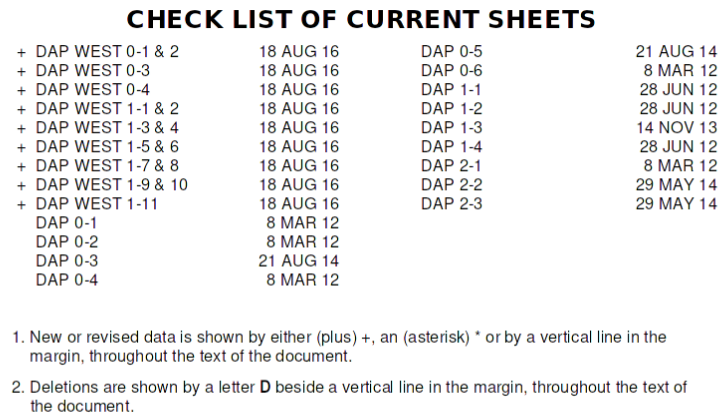
\includegraphics[height=0.42\textheight]{image/dap-diff.png}
\end{block}
\end{frame}

\begin{frame}
\frametitle{Let's fix it}
\begin{block}{I dream of prototyping/proposing such a system}
\begin{itemize}
\item<1-> but from where to source the aeronautical data?
\item<2-> do airservices source it from Geoscience Australia?
\item<3-> and then what?
\item<4-> HALP
\end{itemize}
\end{block}
\end{frame}
